\documentclass{midl} % Include author names
%\documentclass[anon]{midl} % Anonymized submission

% The following packages will be automatically loaded:
% jmlr, amsmath, amssymb, natbib, graphicx, url, algorithm2e
% ifoddpage, relsize and probably more
% make sure they are installed with your latex distribution

\usepackage{mwe} % to get dummy images

% Header for extended abstracts
\jmlrproceedings{MIDL}{Medical Imaging with Deep Learning}
\jmlrpages{}
\jmlryear{2022}

% to be uncommented for submissions under review
\jmlrworkshop{Short Paper -- MIDL 2022 submission}
\jmlrvolume{-- Under Review}
\editors{Under Review for MIDL 2022}

\title[Medical Image Quality Assurance using Deep Learning]{Medical Image Quality Assurance using Deep Learning}

\midlauthor{\Name{{Dž}enan Zukić\nametag{$^{1}$}} \Email{dzenan.zukic@kitware.com}\\
\Name{Anne Haley\nametag{$^{1}$}} \Email{anne.haley@kitware.com}\\
% \Name{Daniel Chiquito\nametag{$^{1}$}} \Email{daniel.chiquito@kitware.com}\\
% \Name{Matt McCormick\nametag{$^{1}$}} \Email{matt.mccormick@kitware.com}\\
\Name{Curtis Lisle\nametag{$^{2}$}} \Email{clisle@knowledgevis.com}\\
\Name{James Klo\nametag{$^{3}$}} \Email{jim.klo@sri.com}\\
\Name{Kilian M. Pohl\nametag{$^{3}$}} \Email{kilian.pohl@stanford.edu}\\
\Name{Hans J. Johnson\nametag{$^{4}$}} \Email{hans-johnson@uiowa.edu}\\
\Name{Aashish Chaudhary\nametag{$^{1}$}} \Email{aashish.chaudhary@kitware.com}\\
\addr $^{1}$ Kitware Inc., Carrboro, North Carolina, USA\\
\addr $^{2}$ KnowledgeVis LLC, Altamonte Springs, Florida, USA\\
\addr $^{3}$ Center for Software Engineering, SRI International, Menlo Park, CA, USA\\
\addr $^{4}$ Electrical and Computer Engineering, University of Iowa, IA, USA\\
\vspace{-2\baselineskip}
}

\begin{document}

\maketitle

\begin{abstract}
We present an open-source web tool for quality control of distributed imaging studies.
To minimize the amount of human time and attention spent reviewing the images,
we created a neural network to provide an automatic assessment.
This steers reviewers' attention to potentially problematic cases,
reducing the likelihood of missing image quality issues.
We test our approach using 5-fold cross validation on a set of 5217 magnetic resonance images.
\end{abstract}

\begin{keywords}
quality control, quality assurance, neural networks, web interface.
\end{keywords}

\section{Introduction}

Discovery of new knowledge in medicine is sometimes accomplished by large, multi-center imaging studies. The success of these studies depends on the quality of images and the resulting measurements. 
%regardless of the size of the study.
% Many studies rely on in-house procedures that combine automatically generated scores with manually guided checks, such as visual inspection. Currently these procedures are often implemented by combining several software systems that are not designed to support Quality Assurance (QA) or Quality Control (QC) processes.
Our open-source \href{https://github.com/OpenImaging/miqa}{Medical Image Quality Assurance} (MIQA) system represents a design that facilitates collaboration and sharing. It incorporates a state-of-the-art deep learning component to improve the effectiveness of Quality Control (QC) efforts unique to the needs of multi-center studies. The usefulness of this unique QC system is being tested by the National Consortium on Alcohol and Neurodevelopment in Adolescence (NCANDA) project. NCANDA uses magnetic resonance images (MRIs) of the brain, so we focus on deep learning for QC of head MRIs in this paper.

MIQA is a client-server web application based on \href{https://github.com/girder/girder}{Girder} and \href{https://www.django-rest-framework.org/}{django}. It uses \href{https://vuejs.org/}{Vue} and \href{https://vuetifyjs.com/}{Vuetify} for its graphical user interface (GUI). For image processing we use the \href{https://itk.org/}{Insight Toolkit (ITK)}. For neural network related operations we use \href{https://pytorch.org/}{PyTorch}, \href{https://monai.io/}{MONAI}, and \href{https://torchio.readthedocs.io/}{TorchIO}.

% Images are either imported or uploaded. During import, images are subjected to NN automatic quality assessment synchronously. After upload, images are auto-assessed asynchronously. Once the assessment is finished, the GUI is updated with the information.
Images are auto-assessed after upload.
% Automatic assessment helps human reviewers.
%% COMMENT: --- The next sentence will not make sense to rmost readers.  Which images are "not reviewed", and what are "tier one reviewers"?
Images which are not reviewed are available in a queue to tier one reviewers. 
%% COMMENT: Who are "They".  The unreviewed images, or the "tier one reviewers", or the "automated review mechansims"?
They can mark it as either good or questionable. Questionable images need to be reviewed by tier two reviewers who then make a final decision. An image can be marked bad only if it has presence of at least one artifact. This can be indicated in the GUI, or in a free-form text comment provided if the problem does not match the predefined artifact classes.

% I would like to mention that we use MRIQC~\cite{esteban2017mriqc}, but we should implement that before the paper deadline.

As far as we know, this is the first attempt at assessing image quality of 3D images. Previous studies used photographs~\cite{bosse2017deep,hosu2020koniq}, retinal fundus images~\cite{yu2017image},
% linguistic descriptions of images~\cite{hou2014blind},
or tried to improve image quality~\cite{higaki2019improvement}. The closest one focuses on quantifying motion artifact \cite{butskova2021adversarial}, but that is only one of nine artifacts we consider here. Their ultimate goal was to correct motion artifacts. % rekik_adversarial_2021

\section{Materials and Methods}

For model training, we use data from the PREDICT-HD study~\cite{paulsen2014clinical}, which has manually assessed quality for structural (T$_1$, T$_2$, PD) brain MRIs. In this study we used only the T$_1$-weighted images. 2299 were acquired on 1.5T and 2918 on 3T MRI machines.
%% COMMENT: Previous sentence should also metntion the number of unique MRI scanners used.  It was around 50 scanners
The most important annotation is overall quality, scored on 0-10 scale (see \figureref{fig:slices}). The original study included manual assessment of signal to noise ratio and contrast to noise ratio. We didn't use these metrics as they are highly correlated the with overall quality, with Pearson coefficients of 0.721 and 0.715, respectively.
% We made no attempt to use free-text comments.

\begin{figure}[btp] %btph
 % Caption and label go in the first argument and the figure contents
 % go in the second argument
\floatconts
  {fig:slices} % Subject 250121, session 91941, run 011.
  {\caption{Left: slices of a T$_1$ weighted image with an overall score of 8 and no artifacts present. All the images from PREDICT-HD set are defaced with a facial blur. Right: confusion matrix for overall quality for fold 3. R$^2$=0.24 (close to average).}}
  {
  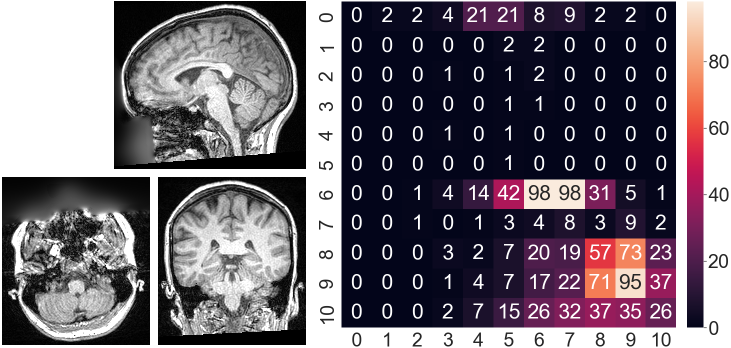
\includegraphics[width=0.75\linewidth]{figure.png}
  \vspace{-1.5\baselineskip} % Since we have no text here, remove one 1.5 lines worth of vertical space
  }
\end{figure}

%% COMMENT:  The provided QC were indications of what was observed.  I would not say that the lack of a positive indication definitively means that absences of the characteristic, just that it was not observed.
% There is not enough space here to squeeze that detail in :D
The PREDICT-HD study data contained nine presence/absence indications of artifacts and one of anatomical variants in the images.
% Some of the images were missing a few of the indications.
Of the 5217 T$_1$ images, 520 indicated normal anatomical variants, 61 indicated lesions, 269 identified as incomplete brain coverage, 30 misalignment, 28 indicated wraparound, 347 ghosting, 585 inhomgeneity, 187 metal susceptibility, 888 flow artifact, and 1286 indicated truncation.

The data largely consisted of images with little or no artifacts. 392 images had quality five or lower (considered bad by PREDICT-HD experimenters), while 4825 had quality six or higher. We augmented the training data to compensate for this class imbalance. For augmentation, we extended the \href{https://torchio.readthedocs.io/transforms/augmentation.html}{TorchIO library} and applied random operations, each with probability ranging from 10\% to 50\%. We implemented \href{https://github.com/OpenImaging/miqa/pull/339}{five simulated artifacts}: ghosting, motion, inhomogeneity, spike, and noise.

Since the images have variable sizes (ranging from 192x256x104 to 512x512x256 here), we decided to split them into tiles of size 64$^3$ with minimal overlap. We apply the neural network (NN) to each tile, and then average the outputs. Our NN has 5 convolutional layers and a fully connected layer with eleven outputs. In the loss function, we combine regression to overall quality with the focal loss for each of the ten presence indicators. For training we use AdamW optimizer and an exponential learning rate schedule. We trained for a preset number of epochs, determined experimentally to allow convergence.


\section{Results and Conclusion}

We split the available data into 5 folds based on subject identifier. We used \href{https://en.wikipedia.org/wiki/Coefficient_of_determination}{coefficient of determination} R$^2$ applied to the overall quality (0-10) to assess predictive power. On validation data, average R$^2$ was 0.26 (see \figureref{fig:slices} for an example) and on training data where it was 0.61. As there are no previous studies to compare to, we are setting precedent.

We provide source at \url{https://github.com/OpenImaging/miqa}, where we openly develop this system. We also maintain a demo instance at \url{https://miqa.miqaweb.io/}.
% Next steps are adding \href{https://github.com/OpenImaging/miqa/pull/441}{permutation and swapping of axes} as an additional augmentation for training, applying this to all 9475 structural images, and transferring this to NCANDA data (which is not defaced).
We welcome collaborative use of this software in medical research and clinical practice.

% Acknowledgments---Will not appear in anonymized version
\midlacknowledgments{We thank our Kitware colleagues: Scott Wittenburg, Daniel Chiquito, Zach Mullen, Matt McCormick, and Jeff Baumes. This work was funded by NIH grant R44MH119022.}

\bibliography{midl-samplebibliography}

\end{document}
